\documentclass{labo}

\usepackage{charter}
\usepackage[utf8x]{inputenc}
\usepackage[T1]{fontenc}
\usepackage{ucs}
\usepackage{amsthm} %numéroter les questions
% \usepackage[frenchb]{babel}
\usepackage{datetime}
\usepackage{xspace} % typographie IN
\usepackage{hyperref}% hyperliens
\usepackage[all]{hypcap} %lien pointe en haut des figures
\usepackage[french]{varioref} %voir x p y
\usepackage{fancyhdr}% en têtes
\usepackage[]{graphicx} %include pictures
% \usepackage{pgfplots}
\usepackage[americanresistors,siunitx]{circuitikz}
\usepackage[]{gnuplottex}
\usepackage{ifthen}
\usepackage{mathastext} % math as standfard text : units are respecting typography conventions.
\usepackage[]{subfig}
\usepackage[]{attachfile}
\usepackage{tikz}
\usetikzlibrary{babel,positioning,calc}
\usepackage{siunitx}
\usepackage{amssymb}
\usepackage{xcolor}
\usepackage{float}
\usepackage[normalem]{ulem}
\usepackage{todonotes}

\usepackage{framed}

%%%%%%%%%%%%
% Tables
%%%%%%%%%%%%
\usepackage{booktabs}
\renewcommand{\arraystretch}{1.1} % Opens up the table a tad
\usepackage{multicol}
\usepackage{multirow}

\newboolean{koriG}
\ifx\koriG\undefined
\correction{false}
\else
\correction{true}
\fi

\newcommand{\itgv}[1]{\ifthenelse{\boolean{corrige}}{{\color{blue}#1}}{}} %si corrigé vrai...
\newcommand{\ifgv}[1]{\ifthenelse{\boolean{corrige}}{}{#1}} %si corrigé vrai...

% \correction{false}
%\correction{true}

\definecolor{darkblue}{rgb}{0,0,0.5}

%% fancy header & foot
\pagestyle{fancy}
\lhead{[EOSI40] Instrumentation labs\\ Lab 3: Rigol DG1022 Signal Generator command}
\rhead{v0.9.0 \\ page \thepage}
\chead{\ifthenelse{\boolean{corrige}}{Corrigé}{}}
\cfoot{}
%%

\author{GEI}


\setlength{\parindent}{0pt}


%from SO: kinky cross for wires
\tikzset{
  declare function={% in case of CVS which switches the arguments of atan2
    atan3(\a,\b)=ifthenelse(atan2(0,1)==90, atan2(\a,\b), atan2(\b,\a));},
  kinky cross radius/.initial=+.125cm,
  @kinky cross/.initial=+, kinky crosses/.is choice,
  kinky crosses/left/.style={@kinky cross=-},kinky crosses/right/.style={@kinky cross=+},
  kinky cross/.style args={(#1)--(#2)}{
    to path={
      let \p{@kc@}=($(\tikztotarget)-(\tikztostart)$),
          \n{@kc@}={atan3(\p{@kc@})+180} in
      -- ($(intersection of \tikztostart--{\tikztotarget} and #1--#2)!%
             \pgfkeysvalueof{/tikz/kinky cross radius}!(\tikztostart)$)
      arc [ radius     =\pgfkeysvalueof{/tikz/kinky cross radius},
            start angle=\n{@kc@},
            delta angle=\pgfkeysvalueof{/tikz/@kinky cross}180 ]
      -- (\tikztotarget)}}}


\begin{document}
\tptitle{}{Lab 3: Rigol DG1022 Signal Generator command}

The objective of this lab is to use SCPI commands to control the signal generator Rigol DG1022.
A command is a particular character string, specifying an instruction and arguments.
Rigol, the device manufacturer, has a detailed documentation about the command syntax that can be used with the DG1000 family.\footnote{The following is an excerpt from “RIGOL Programming Guide, DG1000 Series Dual-Channel Function/Arbitrary Waveform Generator”, RIGOL Technologies, Inc., 2014.}

\begin{leftbar}
{\Large{\textbf{Command Syntax}}}\\
The command systems of DG1000 present a hierarchy structure (tree system) and each command consists of a “Root” keyword and one or multiple sub-keywords. 
The keywords are separated by “:” and are followed by the parameter settings available, “?” is added at the end of the command string to indicate a query and the command and parameter are separated by “space”.\\

For example,\\
FUNCtion:SQUare:DCYCle \{<percent>|MINimum|MAXimum\}\\
FUNCtion:SQUare:DCYCle? [MINimum|MAXimum]

\textbf{FUNCtion} is the root keyword of the command, \textbf{SQUare} and \textbf{DCYCle} are the
second-level and third-level keywords respectively, all the keywords are separated by
“:”. <percent> denotes the parameter that users can set; “?” denotes query; the
command \textbf{FUNCtion:SQUare:DCYCle} and parameter are separated by “space”.\\

“,” is usually used to compare multiple parameters existing in one command, for
example,\\
DATA VOLATILE,<value>,<value>, . . .
\end{leftbar}


To actually use those commands, you will need to handle VIs associated to the character strings.
The commands are then transmitted using the VISA protocol and are found in the functions palette “Instrument I/O > VISA” (see Figure~\ref{fig:visa}).
The first step is to open a communication, then there must be a delay of 150ms between eaach command.
Finally, the communication must be closed.\\

\begin{figure}[ht!]
\centering
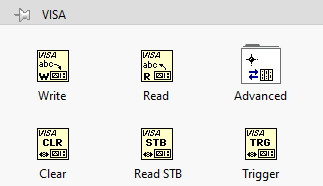
\includegraphics[scale=0.8]{functions-palette-visa.png}
\caption{VISA functions palette for the block diagram.}
\label{fig:visa}
\end{figure}

To handle character strings, a particularly useful block is the “String > Additional String Functions > Pick Line” (see Figure~\ref{fig:palette-string}) to allow the user to choose between several options through the front panel.\\

\begin{figure}[ht!]
\centering
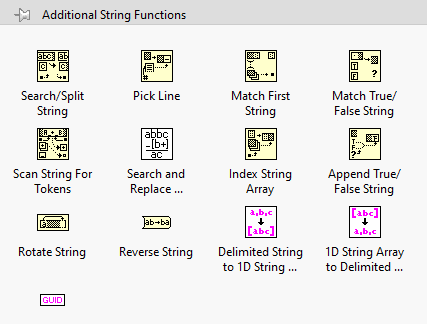
\includegraphics[scale=0.8]{functions-palette-additional-string.png}
\caption{Additional string functions palette for the block diagram, in which can be found the “Pick Line” block.}
\label{fig:palette-string}
\end{figure}

An other block can convert digital data into character strings for the user interface, using the following convention and the “Format Into String” block (see Figure~\vref{fig:format-into-string}):
\begin{itemize}
  \item Specify a character for the decimal separator
  \item Send a string linked to the command (with a space at the end)
  \item Format the number at the input of the block into fract/sci notation
\end{itemize}
All of those parameters can be set through the “Edit Format String” interface opened by double-clicking on the block (see Figure~\vref{fig:format-into-string-edit}).

\begin{figure}[ht!]
\centering
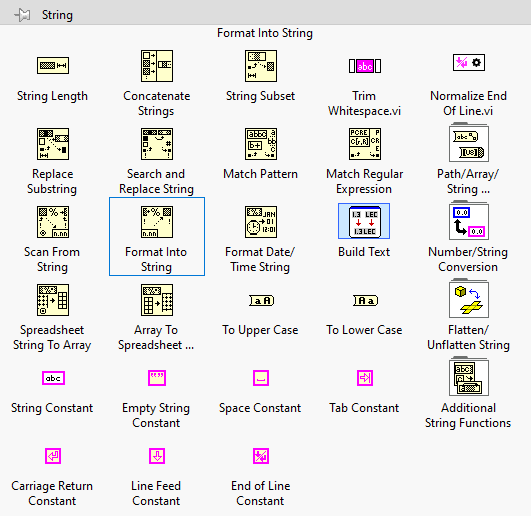
\includegraphics[scale=0.8]{functions-palette-fromat-into-string.png}
\caption{“String” functions palette for the block diagram.}
\label{fig:format-into-string}
\end{figure}

\begin{figure}[ht!]
\centering
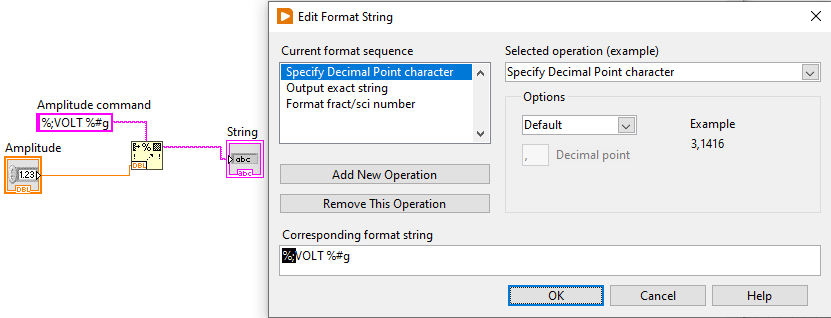
\includegraphics[width=\textwidth]{format-into-string-edit.png}
\caption{String format editor and block diagram converting a simple double value into a string “VOLT <value>”.}
\label{fig:format-into-string-edit}
\end{figure}



\section{Activation interface for the Rigol generator}
Install the drivers for the device first.
In LabView, navigate through the menus “Tools > Instrumentation > Find Instrument Drivers...” which lands you on a window similar to Figure~\ref{fig:labview-driver-finder}.
Click the “Search >” button, select “rgdg1xxx Instrument Driver” and click on “Install >”\footnote{You might need to be logged in into your NI account for the search function to be available.}.
You may find the device specific blocks in “Instrument I/O > Instr Drivers > RIGOL DG1000 Series”.

\begin{figure}[ht!]
\centering
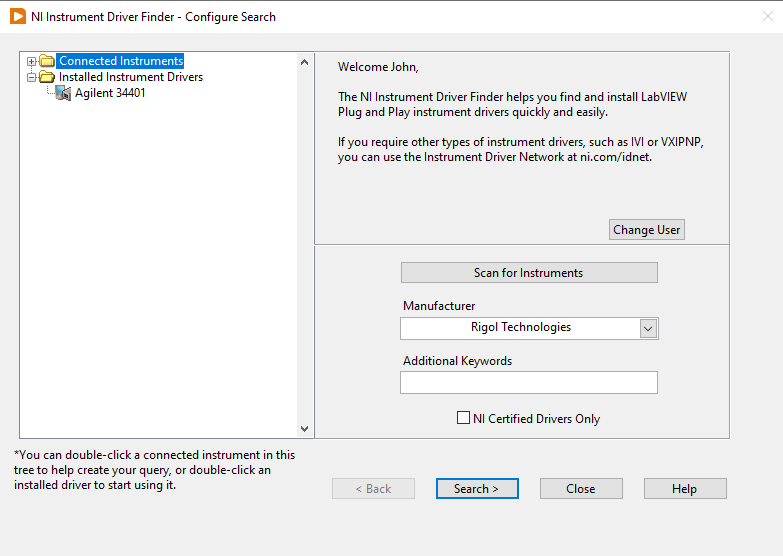
\includegraphics[scale=.7]{LabView-driver-finder.png}
\caption{LabView driver finder tool.}
\label{fig:labview-driver-finder}
\end{figure}

Using VISA blocks and SCPI commands, build an interface that allows the user to enable or disable the channels of the generator\footnote{the RIGOL driver blocks already exist to vastly simplify the task, but we won't use them at the moment for the sake of the exercise.}.
Figure~\vref{fig:block-diagram-channel} exploits event and boolean structures to do so, may it inspire you to add a second channel.

\begin{figure}[ht!]
\centering
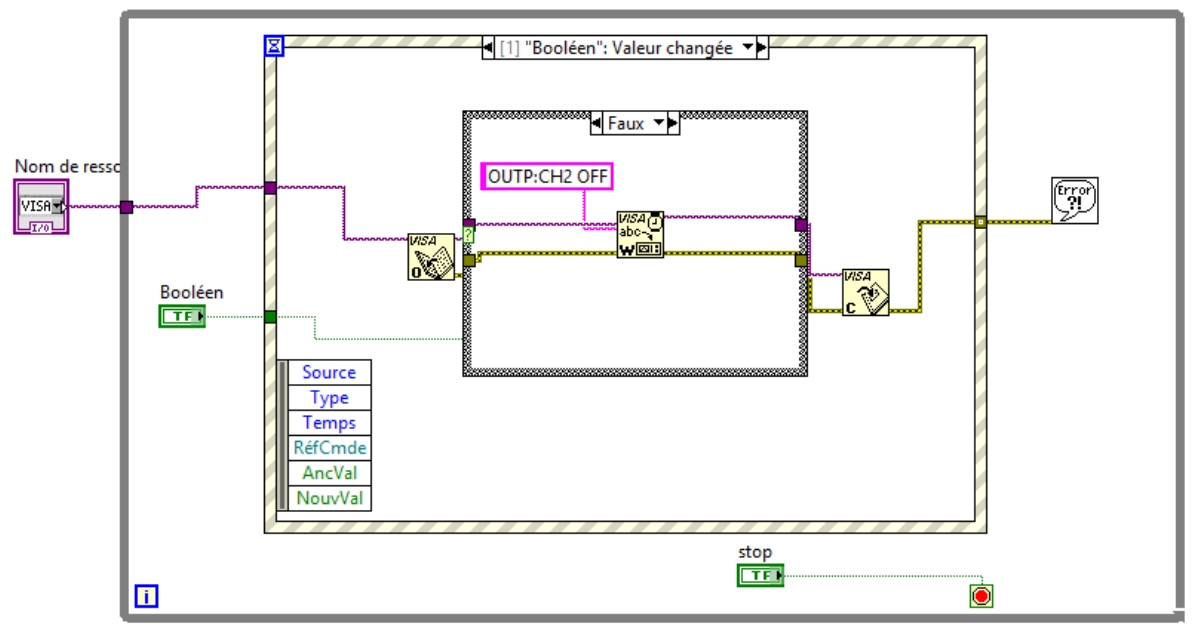
\includegraphics[width=\linewidth]{block-diagram-channel.png}
\caption{Block diagram of a program controlling a single channel of the signal generator.}
\label{fig:block-diagram-channel}
\end{figure}


\section{Rigol DG1022 Interface -- The Remake}
Build an interface that allows to configure the Rigol generator settings, similar to Figure~\vref{fig:front-panel-Rigol}:
\begin{itemize}
  \item Waveform function
  \item Amplitude
  \item Peak-to-peak voltage
  \item DC offset
  \item Frequency
  \item Duty cycle in case of a square signal
\end{itemize}
A ``configure'' button should allow the user to update the configuration.
The buttons to control the channels activation should also be reused.

Implement one feature at a time and remember that you can nest your VIs.

\begin{figure}[ht!]
\centering
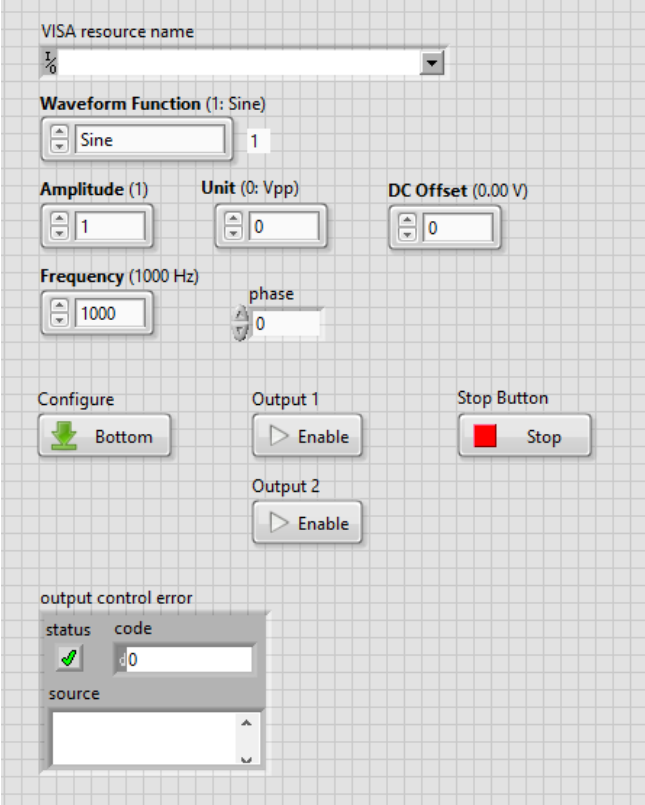
\includegraphics[width=.5\linewidth]{front-panel-Rigol.png}
\caption{Front panel view of a VI emulating the DG1022 physical interface.}
\label{fig:front-panel-Rigol}
\end{figure}


\section{Sweep that frequency}
Implement a frequency sweep feature with options similar to what the generator already offers.
In particular, the user should be able to change the sweep progression from linear to logarithmic, the start and stop frequency, as well as the total duration of one sweep cycle.

\section{Sweep anything, really}
Strong with your experience from the previous exercise, implement a sweep feature for any setting, such as the signal amplitude, duty cycle, phase, offset, etc.

Check the result using the oscilloscope.



% \section{Oscilloscope interface}



% \section{Interconnect both devices}



\section{Bonus: Validation testing}
Validate your configuration of the generator by reading the device registers and display the result of this validation.






% \begin{figure}[ht!]
% \centering
% 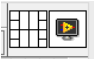
\includegraphics[]{mod-icon-conn.png}
% \caption{}\label{fig:mod-icon-conn}
% \end{figure}



% \Question{}{}
\end{document}
